\documentclass{article}
\usepackage[a4paper, margin=2.5cm]{geometry}
\usepackage{polski, graphicx, float, siunitx}
\setcounter{secnumdepth}{0}

\begin{document}
\subsection{Przetwornica 12V na 5V}
\subsubsection{Zastosowanie}
Z powodu dodania paska LED, który wymaga zasilania 5V oraz prądów rzędu 2A, zdecydowano się na samodzielne zaprojektowanie przetwornicy 12V na 5V, gdyż gotowe moduły
psułyby estetykę zegara. Nie zastosowano również stabilizatora liniowego, gdyż było by to nieefektywne i wymagało dodatkowego radiatora.
\\\\
Zdecydowano się na przetwornicę impulsową, która jest znacznie bardziej efektywna. Dzięki temu również można było zminimalizować straty mocy na zasilaniu linii 3.3V, ponieważ
można było zastosowac LDO zamiast stabilizatora liniowego z 12V na 3.3V.

\subsubsection{Wybór układu scalonego}
Zdecydowano się na układ TPS563219ADDFR produkcji Texas Instruments, który jest przetwornicą impulsową z wbudowanym tranzystorem mocy oraz zapewniajacym prąd wyjściowy do 3A przy 
napięciu wyjściowym do 7V. Układ jest też w obudowie na tyle dużej, by móc go polutować ręcznie. Układ posiada soft-start oraz wyjście power good (potwierdzające start przetwornicy), co nie jest potrzebne w tym zastosowaniu, tak samo 
nie jest to najmniejszy układ, ale zapewnia to łatwość montażu co jest ważne w tym przypadku.

\subsubsection{Założenia projektowe}
% obliczenia szacowanego prądu ledów i reszty komponentów
\begin{itemize}
    \item Napięcie wejściowe: 12V
    \item Napięcie wyjściowe: 5V
    \item Prąd wyjściowy: 2A
    \item 50mV tętnienia napięcia wyjściowego
\end{itemize}


\subsubsection{Dobór cewki}
Dobór cewki wykonano na podstawie tabeli zamieszczonej w dokumentacji układu.
\begin{figure}[H]
    \centering
    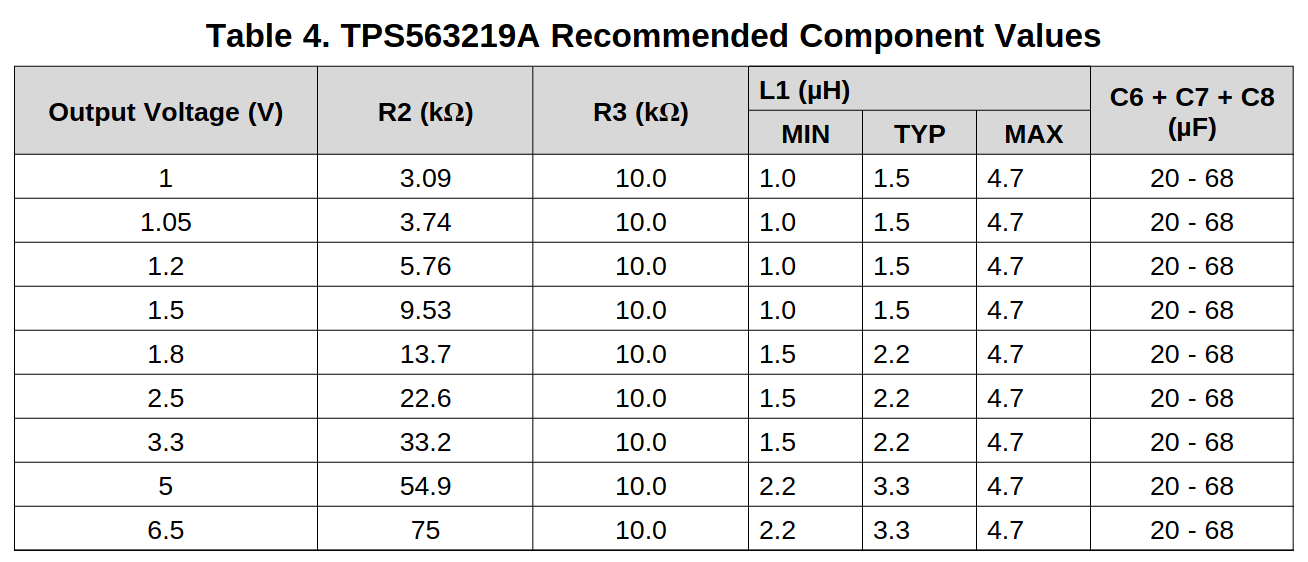
\includegraphics[width=0.8\textwidth]{conv-table.png}
    \caption{Tabela doboru komponentów z noty katalogowej}
\end{figure}



\subsubsection{Schemat}
\begin{figure}[H]
    \centering
    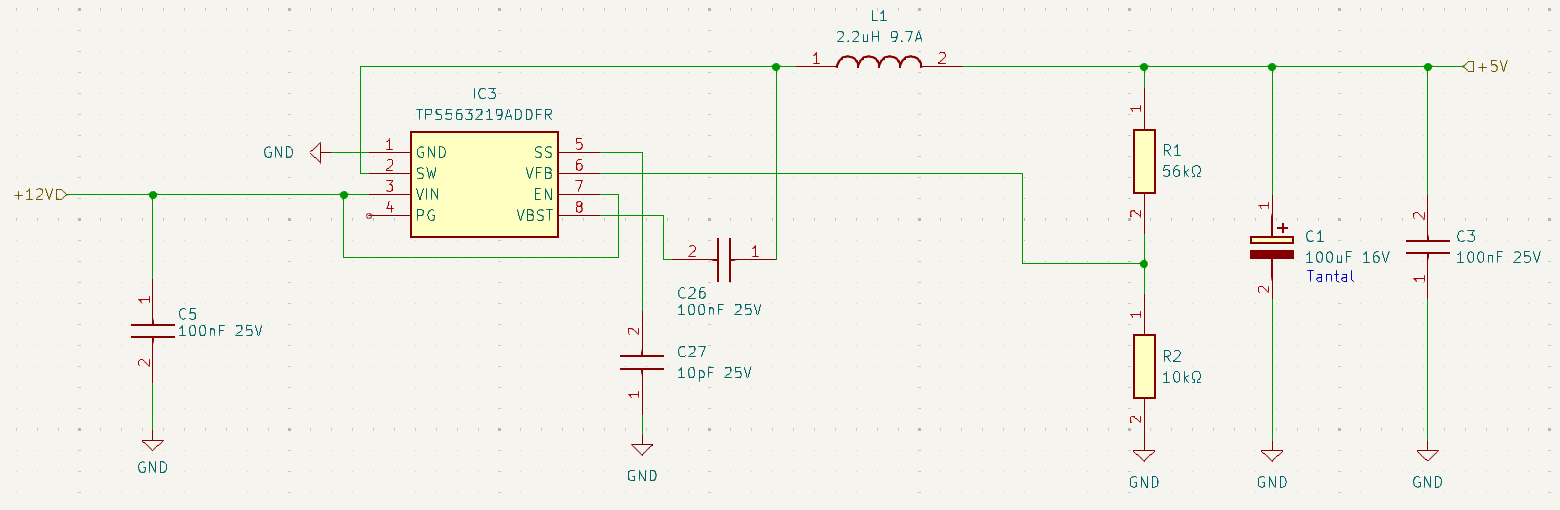
\includegraphics[width=0.8\textwidth]{12V_to_5V_conv_schemat.png}
    \caption{Schemat złącza DC-Plug}
\end{figure}

\end{document}
